\documentclass[12pt,oneside]{book}
\usepackage{geometry}                		% See geometry.pdf to learn the layout options. There are lots.
\geometry{a4paper}                   			% ... or a4paper or a5paper or ... 
%\geometry{landscape}                		% Activate for for rotated page geometry
%\usepackage[parfill]{parskip}    		% Activate to begin paragraphs with an empty line rather than an indent
\usepackage{graphicx}				% Use pdf, png, jpg, or epsß with pdflatex; use eps in DVI mode
								% TeX will automatically convert eps --> pdf in pdflatex		
\usepackage{amssymb}

\usepackage[spanish]{babel}			% Permite que partes automáticas del documento aparezcan en castellano.
\usepackage[utf8]{inputenc}			% Permite escribir tildes y otros caracteres directamente en el .tex
\usepackage[T1]{fontenc}				% Asegura que el documento resultante use caracteres de una fuente apropiada.

\usepackage{hyperref}				% Permite poner urls y links dentro del documento

\title{Manual de Juego Sudoku}
\author{Manuel Suárez-Veronica Pozo-José Salas}
%\date{}							% Activate to display a given date or no date

\begin{document}
\maketitle
\tableofcontents

\chapter{Introducción}
El libro a continuación es creado como una herramienta para el desarrollo de habilidades de edición colaborativa de documentos de texto plano. La herramienta que habilita dicha colaboración, en este taller, es Git pero podría ser reemplazada por otros sistemas de versionamiento.

\chapter{El Juego}

\chapter{Historia}
El Sudoku puede haberse ideado a partir de los trabajos del matemático suizo Leonhard Euler (1707-1783), quién utilizó los cuadrados latinos1 para realizar cálculos probabilísticos, aunque su aparición más obvia se dio en el año 1979, cuando el norteamericano Howard Garns publica en Nueva York, a través de la empresa Dell Magazines, un juego muy similar conocido bajo el nombre de “Number Place”. En el año 1984 una editorial japonesa lo exportó hacia ese país, divulgándolo en el periódico “Monthly Nikolist” bajo el nombre de “Los números deben estar solos” (cuyo apócope en japonés es SuDoku). La editorial introdujo con el correr de los años algunas innovaciones que hicieron que el juego ganara gran popularidad entre los lectores. 
Sus inicios reales como Sudoku en Occidente se remontan a los años 2004/2005, gracias a su publicación en los diarios “The Times” y “The Daily Mail”. Desde aquel entonces, el juego ha alcanzado una gran popularidad en el mundo moderno: en 2005 se publicó el primer libro acerca de Sudokus en el mundo (“Los mejores Sudokus”, con 200 tableros agrupados en 4 niveles de dificultad) y se lo incluyó entre los 9 problemas del ICPC (sigla de International Collegiate Programming Contest). 
\chapter{Aplicacion}
	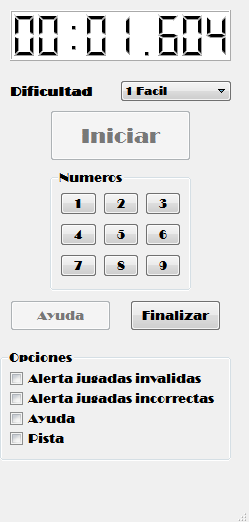
\includegraphics[width=1.10\textwidth]{./imagenes/Panel_izquierdo.png}
	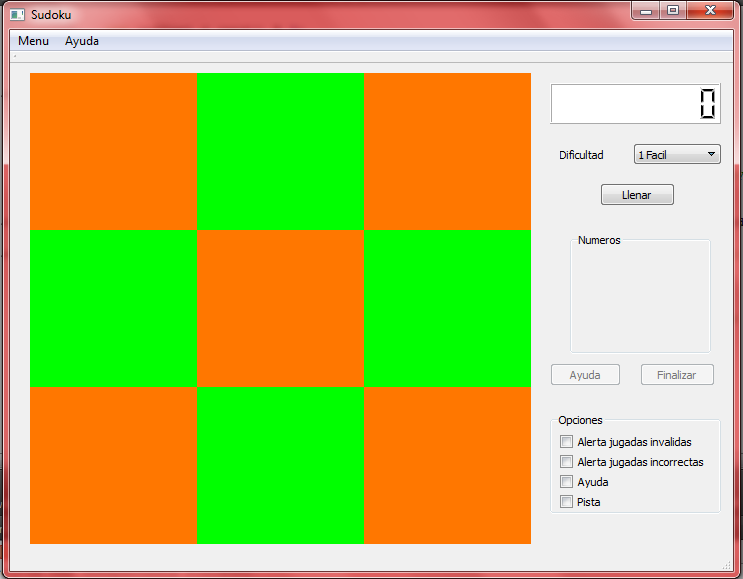
\includegraphics[width=1.10\textwidth]{./imagenes/PantallaPrincipal.png}
\chapter{Funcionalidad}
\begin{center} Generacion de tableros:\end{center}
\begin{itemize}
\item  Algoritmo implementado.
\begin{itemize}
	\item Se genera un tablero con numeros random hasta que este sea resolvible.
	\item Se verifica si es resolvible.
	\item Se trata de resolver por arreglos de posibildades de numeros en casillas.
	\item Si no se puede resolver así, se utiliza la técnica del Backtracking. 
	\item Utizando Backtracking se busca solucionar cambiando los numeros detras del vacio, y utilizando recursion de la misma.
	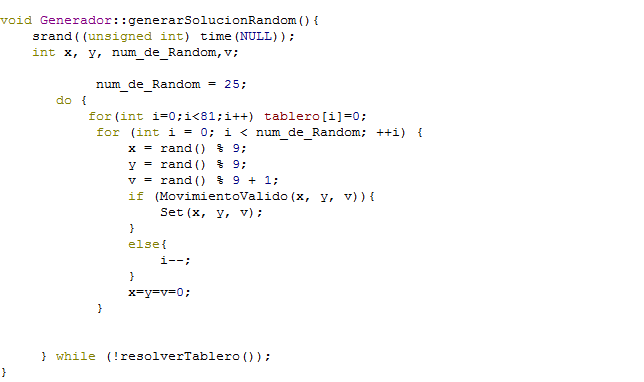
\includegraphics[width=1.10\textwidth]{./imagenes/codigo_genrador.png}
\end {itemize}

\item  Dificultad.
\begin {itemize}
	\item Se procede a quitar numeros del arreglo, y comprobar si se puede resolver y tienen única solución.
	\item Se agregan en un pila los numeros y posiciones que fueron quitadas y se podia obtener única solución.
	\item Segun el numero de dificultad se obtienen posiciones random repetidamente tantas casillas hay, y se ve las veces 
	que puede estar ese numero.


	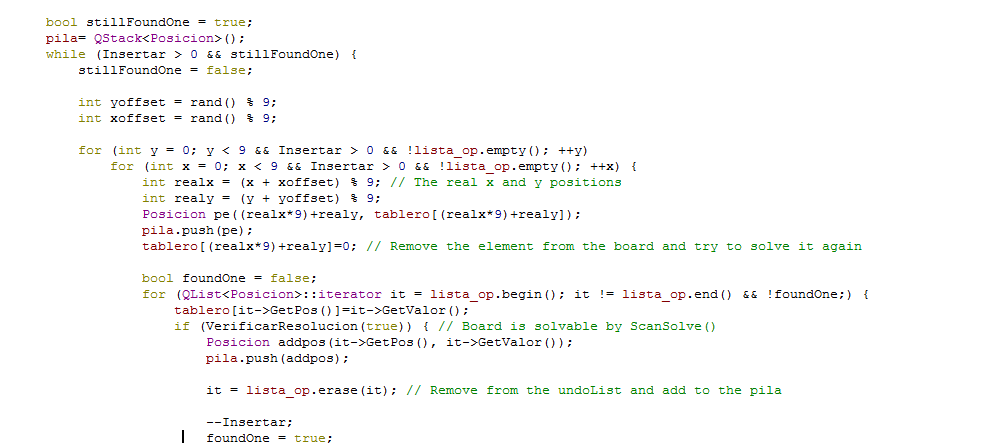
\includegraphics[width=1.10\textwidth]{./imagenes/Codigo_dificultad.png}
\end {itemize}
\item  Guardar y cargar tableros cifrados .
	
\item   Jugar y finalizar juego (2).
\item   Puntaje (3).
\end{itemize}
\chapter{Colaboraciones}
Correcta documentación de colaboración otorga
puntaje.
• Si la documentación es inconsistente con una
distribución adecuada de trabajo se considerará
descontar puntos.
• Contabilicen número de commits por integrante.
• ¿En qué fechas hay picos?
\chapter{Conclusiones}
Se concluye
\end{document}  
